\documentclass[conference]{IEEEtran}
\IEEEoverridecommandlockouts
\usepackage{cite}
\usepackage{amsmath,amssymb,amsfonts}
\usepackage{graphicx}
\usepackage{textcomp}
\usepackage{xcolor}
\usepackage{hyperref}
\usepackage{booktabs}

\def\BibTeX{{\rm B\kern-.05em{\sc i\kern-.025em b}\kern-.08em
    T\kern-.1667em\lower.7ex\hbox{E}\kern-.125emX}}
\begin{document}

\title{Clasificación de Plancton mediante Deep Learning: Comparativa de Arquitecturas\\}

\author{\IEEEauthorblockN{Daniel Martín Pérez}
\IEEEauthorblockA{\textit{Máster Universitario en Investigación en Inteligencia Artificial (MUIIA)} \\
\textit{Asignatura: Deep Learning}\\
dmarper2@upo.es}
}

\maketitle

\begin{abstract}
Este trabajo presenta la clasificación de imágenes microscópicas de plancton mediante tres arquitecturas de aprendizaje profundo: un Perceptrón Multicapa (MLP), una Red Neuronal Convolucional diseñada desde cero (Custom CNN) y un modelo basado en Transfer Learning (MobileNetV2). El dataset presenta un fuerte desequilibrio entre clases, que se ha tratado mediante pesos compensatorios y Data Augmentation. Para evaluar los errores según su gravedad biológica se ha empleado una función de Pérdida Jerárquica que penaliza más las confusiones entre especies de distintos grupos funcionales. Los resultados muestran que el MLP no logra captar los patrones espaciales de las imágenes (57.3\% Accuracy), mientras que la CNN Custom alcanza un 87.2\% y MobileNetV2 un 89.5\%, superando ambas el baseline exigido.
\end{abstract}

\begin{IEEEkeywords}
Deep Learning, Computer Vision, Transfer Learning, CNN, Plancton
\end{IEEEkeywords}

\section{Introducción}
La clasificación de especies de plancton tiene una importancia directa en la vigilancia del estado de los ecosistemas marinos, ya que el plancton es un indicador sensible de cambios ambientales. La identificación manual de estas especies resulta lenta y poco escalable, lo que hace interesante la aplicación de técnicas de Deep Learning para automatizar este proceso.

El dataset empleado contiene imágenes microscópicas en escala de grises de 15 clases de plancton agrupadas en varios Grupos Funcionales. Este conjunto de datos plantea dos retos principales. Primero, existe un claro desequilibrio de clases: algunas especies tienen miles de muestras mientras que otras apenas cuentan con unas decenas. Segundo, los errores de clasificación no tienen todos el mismo coste: confundir dos especies del mismo grupo funcional es menos grave (coste 0.3) que confundir especies de grupos distintos (coste 1.0).

El objetivo del trabajo es diseñar modelos que superen el baseline definido por la asignatura: un Accuracy superior a 0.80 y una Pérdida Jerárquica inferior a 0.85.

\section{Métodos y Arquitecturas}
Se han evaluado tres arquitecturas en las mismas condiciones para poder comparar sus capacidades de forma justa.

\subsection{Preprocesamiento y Balanceo}
Todas las imágenes se redimensionaron a 128$\times$128 píxeles y se normalizaron al rango [0, 1]. Se eligió esta resolución porque conserva suficiente detalle morfológico sin consumir demasiada memoria, lo que permite trabajar con batches de 32 muestras sin problemas.

Para compensar el desequilibrio de clases se calcularon pesos inversamente proporcionales a la frecuencia de cada clase mediante \texttt{sklearn.utils.class\_weight}. De esta forma, durante el entrenamiento el modelo recibe una penalización mayor cuando falla en las clases minoritarias, evitando que se limite a predecir siempre las clases más frecuentes.

Además, se aplicó Data Augmentation (giros horizontales y verticales, rotaciones de hasta 20\degree{} y zoom aleatorio) para generar variaciones de las imágenes de entrenamiento. Esto resulta especialmente útil con las clases menos representadas, ya que amplía artificialmente su variedad visual.

\subsection{Aproximación 1: Perceptrón Multicapa (MLP)}
El MLP se incluyó como modelo de referencia, sabiendo que un modelo basado solo en capas densas no aprovecha la información espacial de las imágenes. La imagen se aplana a un vector de 49.152 valores que pasa por tres capas densas (1024, 512 y 256 neuronas) con capas de Dropout (0.3 y 0.4) para reducir el sobreajuste.

El entrenamiento se detuvo tras 28 épocas porque la precisión de validación no mostró mejoras significativas tras las épocas iniciales. Esto era esperable: al aplanar la imagen, el MLP pierde toda noción de bordes, formas y texturas que son fundamentales para distinguir entre especies.

\begin{figure}[htbp]
\centerline{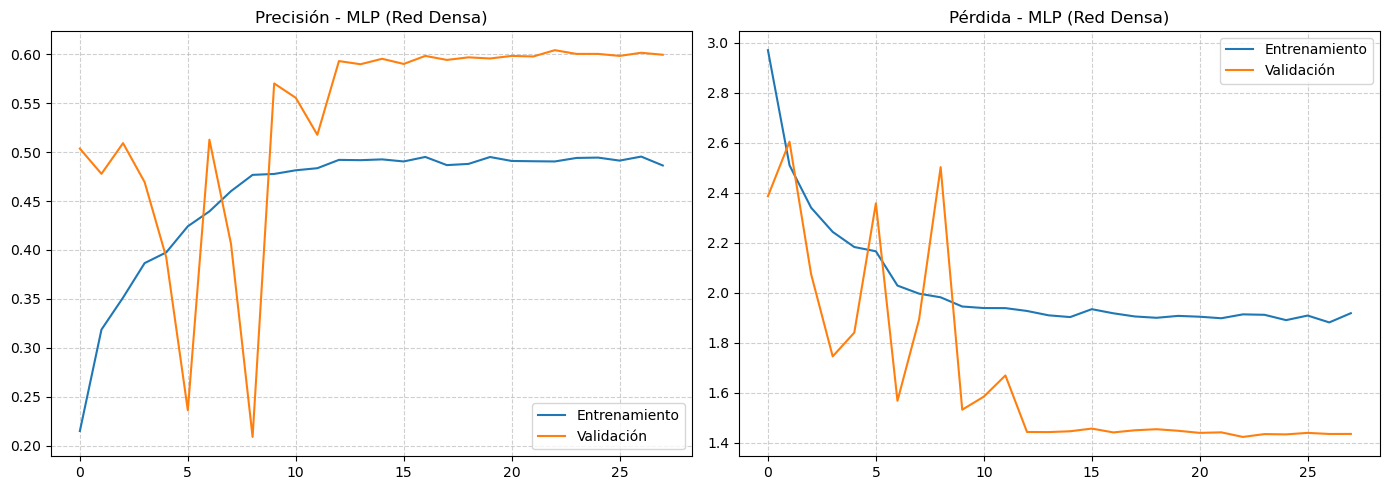
\includegraphics[width=0.48\textwidth]{MLP.png}}
\caption{Curvas de entrenamiento del MLP. Se observa que la pérdida de validación (línea naranja) se mantiene alta sin converger, mientras que la precisión se estanca en torno al 57\%. El modelo no consigue aprender patrones útiles de las imágenes.}
\label{fig:mlp}
\end{figure}

\subsection{Aproximación 2: Custom CNN}
Se diseñó una red convolucional con tres bloques de convolución progresivos (32, 64 y 128 filtros). Se eligió esta progresión porque permite a las primeras capas detectar bordes simples y a las posteriores combinar esos bordes en patrones más complejos como siluetas o texturas.

Cada bloque incluye Batch Normalization antes de la activación (para estabilizar los gradientes y acelerar la convergencia) y MaxPooling para reducir las dimensiones espaciales. Al final, una capa densa con regularización L2 y Dropout del 50\% evitan que la red memorice las muestras de entrenamiento. Las capas convolucionales se inicializaron con He Normal, una técnica recomendada para activaciones ReLU porque mantiene la varianza de las señales estable a lo largo de la red.

Se utilizó AdamW como optimizador porque, a diferencia de Adam estándar, aplica el factor de decaimiento de pesos de forma desacoplada, lo que produce una regularización más limpia. El entrenamiento se detuvo en la época 40 por Early Stopping, al no mejorar la validación de forma sostenida.

\begin{figure}[htbp]
\centerline{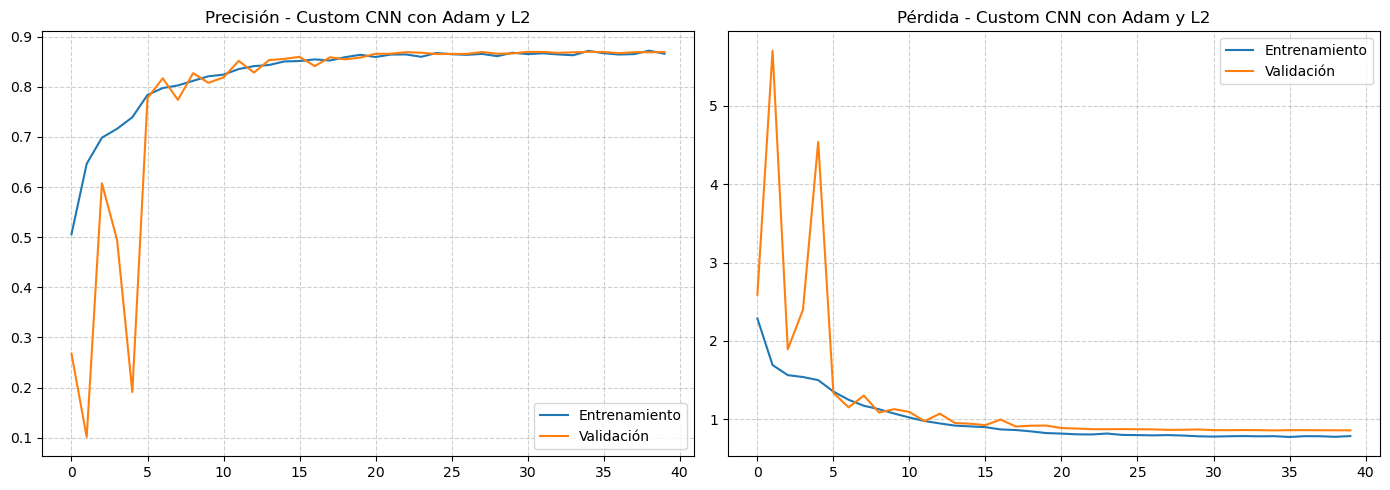
\includegraphics[width=0.48\textwidth]{CNN.png}}
\caption{Curvas de la CNN Custom. A diferencia del MLP, las curvas de entrenamiento y validación convergen de forma paralela, lo que indica que la red generaliza bien. La precisión de validación llega a un 87\% en 40 épocas.}
\label{fig:cnn}
\end{figure}

\subsection{Aproximación 3: MobileNetV2 (Transfer Learning)}
MobileNetV2 es una arquitectura ligera pre-entrenada en ImageNet (millones de imágenes naturales). Se eligió esta red por dos razones: sus bloques residuales invertidos son computacionalmente eficientes, y sus filtros ya reconocen patrones visuales generales (bordes, texturas, formas) que también aparecen en las imágenes de plancton.

El entrenamiento se realizó en dos fases. En la Fase 1 se congelaron todos los pesos de MobileNetV2 y solo se entrenó la cabeza de clasificación nueva (una capa densa + softmax). Esto permitió que la red aprendiera a mapear las características ya extraídas hacia nuestras 15 clases sin destruir los pesos pre-entrenados. En la Fase 2 se descongelaron las últimas 60 capas y se re-entrenó todo junto con una tasa de aprendizaje muy baja ($10^{-5}$) para ajustar de forma gradual los filtros profundos al dominio específico del plancton.

\begin{figure}[htbp]
\centerline{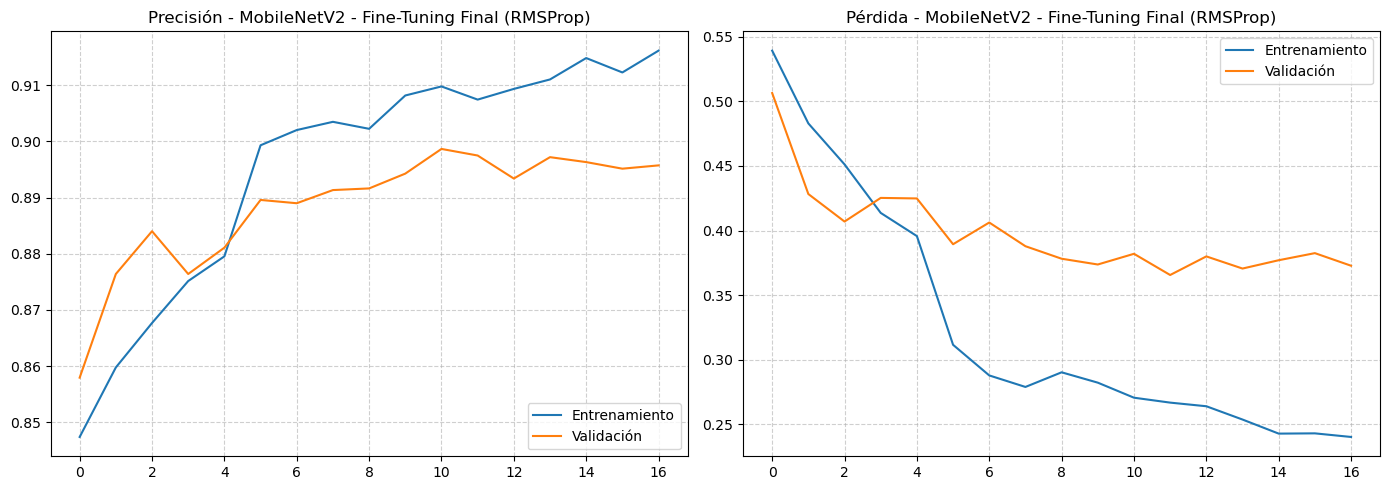
\includegraphics[width=0.48\textwidth]{TL.png}}
\caption{Curvas de MobileNetV2. Se distingue una primera fase donde la pérdida baja rápido (solo se entrena la cabeza) y una segunda fase de fine-tuning donde las curvas se afinan. La precisión final de validación alcanza el 89\%.}
\label{fig:tl}
\end{figure}


\section{Resultados}
La Tabla \ref{tab1} resume el rendimiento final de cada modelo evaluado sobre el conjunto de test reservado.

\begin{table}[htbp]
\caption{Resultados finales sobre el conjunto de test}
\begin{center}
\begin{tabular}{|l|c|c|c|c|}
\hline
Modelo & Épocas & Loss Jerárquica & Accuracy & Estado \\
\hline
(Baseline exigido) & -- & 0.850 & 0.8000 & Objetivo \\
\hline
MLP (Red Densa) & 28 & 1.3575 & 0.5731 & No superado \\
Custom CNN & 40 & 0.8378 & 0.8725 & Superado \\
MobileNetV2 & 17 & 0.3585 & 0.8957 & Superado \\
\hline
\end{tabular}
\label{tab1}
\end{center}
\end{table}

El MLP obtuvo un 57.3\% de Accuracy y una pérdida jerárquica de 1.35, muy lejos del baseline. Esto confirma que sin convoluciones, la red no puede extraer patrones relevantes de las imágenes. La Custom CNN superó el baseline tanto en Accuracy (87.2\%) como en Loss Jerárquica (0.83), demostrando que una arquitectura convolucional bien diseñada es capaz de aprender las características morfológicas del plancton en las 40 épocas de entrenamiento. MobileNetV2 obtuvo los mejores resultados (89.5\% Accuracy, 0.35 Loss) porque ya partía de filtros que entienden patrones visuales generales y solo necesitó adaptarlos al dominio concreto.

\begin{figure}[htbp]
\centerline{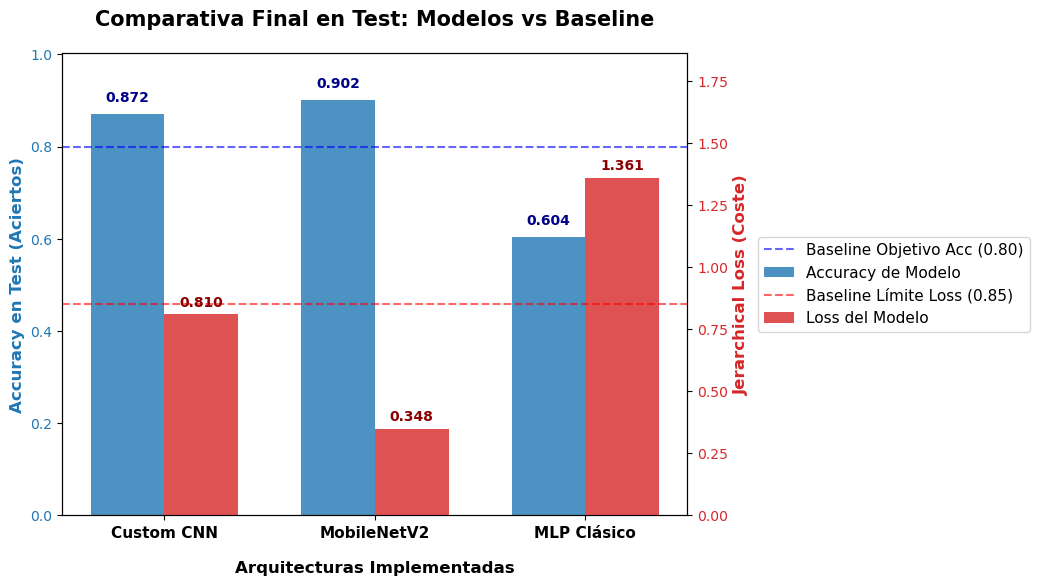
\includegraphics[width=0.48\textwidth]{comparativa.png}}
\caption{Comparativa de los tres modelos frente al baseline. Las barras verdes indican modelos que superan los umbrales exigidos. Se aprecia la diferencia clara entre el MLP y las dos arquitecturas convolucionales.}
\label{fig:comparacion_test}
\end{figure}

\section{Conclusiones}
Este trabajo muestra que las redes convolucionales son la herramienta adecuada para clasificar imágenes de plancton, mientras que una red densa sin convoluciones no es capaz de resolver esta tarea. Los dos modelos basados en convoluciones superaron los umbrales exigidos por el baseline.

La Custom CNN demostró que un diseño cuidadoso con regularización (L2, Dropout, Batch Normalization) y una buena inicialización de pesos puede producir resultados competitivos sin necesidad de recurrir a modelos externos. Por su parte, MobileNetV2 confirmó que reutilizar conocimiento aprendido en otros dominios reduce el tiempo de entrenamiento y mejora los resultados, lo que resulta especialmente valioso cuando el dataset es limitado o desequilibrado.

La principal dificultad del proyecto fue integrar la función de pérdida jerárquica dentro del grafo de TensorFlow de forma compatible con los tensores internos, así como ajustar los pesos de clase para que el entrenamiento no colapsara a favor de las categorías mayoritarias.

\section{Enlaces}
Enlace al Notebook Original de Google Colaboratory y al Vídeo:

\url{}
\url{}

\end{document}
